\documentclass[tikz,border=2pt]{standalone}
\usepackage{amsmath,amssymb}
\usepackage[scaled=0.92]{helvet}
\renewcommand{\familydefault}{\sfdefault}
\usetikzlibrary{positioning,calc,arrows.meta,fit,backgrounds}
\definecolor{seed}{HTML}{2a78d6}
\definecolor{hit}{HTML}{1baf7a}
\definecolor{item}{HTML}{eb6834}
\definecolor{rel}{HTML}{6250d6}
\definecolor{ink}{HTML}{333333}
\definecolor{mute}{HTML}{8a8a85}
\tikzset{
  box/.style={draw=#1,fill=#1!10,rounded corners=1.5pt,minimum height=4.2mm,inner sep=1.6pt,font=\scriptsize,text=ink},
  lab/.style={font=\scriptsize\bfseries,text=ink},
  note/.style={font=\tiny,text=mute,align=left},
  arr/.style={-{Stealth[length=1.6mm]},draw=ink,line width=.5pt},
}
\begin{document}
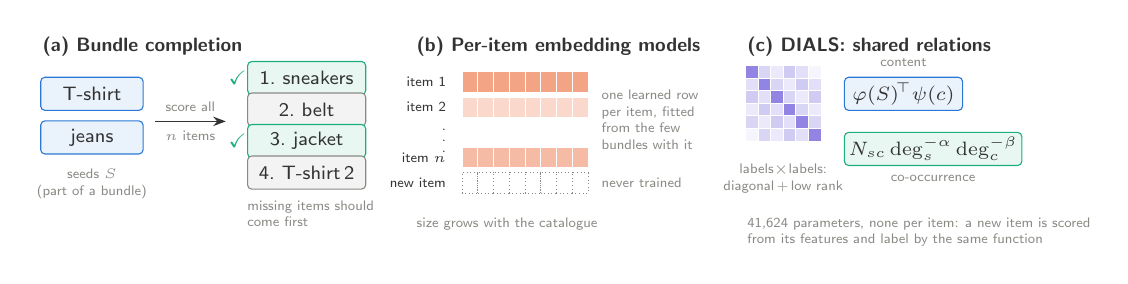
\begin{tikzpicture}
% ---------------- (a) the task ----------------
\node[lab,anchor=west] at (0,2.55) {(a) Bundle completion};
\node[box=seed,minimum width=13mm] (s1) at (0.75,1.95) {T-shirt};
\node[box=seed,minimum width=13mm,below=1.2mm of s1] (s2) {jeans};
\node[note,below=0.6mm of s2,align=center] (sl) {seeds $S$\\(part of a bundle)};
\draw[arr] (1.55,1.6) -- node[above,note]{score all} node[below,note]{$n$ items} (2.45,1.6);
\foreach \t/\c/\y [count=\i] in {sneakers/hit/2.15,belt/mute/1.75,jacket/hit/1.35,T-shirt\,2/mute/0.95}{
  \node[box=\c,minimum width=15mm,anchor=west] (r\i) at (2.72,\y) {\i.~\t};
}
\node[note,anchor=north west] at (2.6,0.72) {missing items should\\come first};
\node[font=\scriptsize,text=hit] at (2.6,2.15) {\checkmark};
\node[font=\scriptsize,text=hit] at (2.6,1.35) {\checkmark};

% ---------------- (b) per-item models ----------------
\begin{scope}[xshift=4.75cm]
\node[lab,anchor=west] at (0,2.55) {(b) Per-item embedding models};
\foreach \y/\t/\f in {2.1/item 1/item,1.78/item 2/item,1.46/$\vdots$/white,1.14/item $n$/item}{
  \node[font=\tiny,text=ink,anchor=east] at (0.62,\y) {\t};
}
\foreach \y/\o in {2.1/60,1.78/25,1.14/45}{
  \foreach \x in {0,...,7}{\fill[item!\o!white,draw=white,line width=.3pt] (0.7+0.2*\x,\y-0.13) rectangle ++(0.2,0.26);}
}
\foreach \x in {0,...,7}{\draw[mute,densely dotted,line width=.3pt,fill=white] (0.7+0.2*\x,0.69) rectangle ++(0.2,0.26);}
\node[font=\tiny,text=ink,anchor=east] at (0.62,0.82) {new item};
\node[note,anchor=west] at (2.35,1.62) {one learned row\\per item, fitted\\from the few\\bundles with it};
\node[note,anchor=west] at (2.35,0.82) {never trained};
\node[note,anchor=north west] at (0.0,0.5) {size grows with the catalogue};
\end{scope}

% ---------------- (c) DIALS ----------------
\begin{scope}[xshift=8.95cm]
\node[lab,anchor=west] at (0,2.55) {(c) DIALS: shared relations};
% label x label relation
\foreach \i in {0,...,5}{\foreach \j in {0,...,5}{
  \pgfmathsetmacro{\o}{ifthenelse(\i==\j,70,mod(\i*7+\j*3,5)*6+6)}
  \fill[rel!\o!white,draw=white,line width=.3pt] (0.1+0.16*\j,2.15-0.16*\i) rectangle ++(0.16,0.16);
}}
\node[note,anchor=north,align=center] at (0.58,1.18) {labels$\times$labels:\\diagonal\,+\,low rank};
% content and graph, stacked
\node[box=seed,minimum width=15mm,anchor=west] (c1) at (1.35,1.95) {$\varphi(S)^{\!\top}\psi(c)$};
\node[note,anchor=south] at (c1.north) {content};
\node[box=hit,minimum width=15mm,anchor=west] (g1) at (1.35,1.25) {$N_{sc}\deg_s^{-\alpha}\deg_c^{-\beta}$};
\node[note,anchor=north] at (g1.south) {co-occurrence};
\node[note,anchor=north west] at (0.0,0.5) {41,624 parameters, none per item: a new item is scored\\from its features and label by the same function};
\end{scope}
\end{tikzpicture}
\end{document}
